\runningheader{Mathematics 6}{Unit Practice Set}{Page \thepage\ of \numpages}

\begingradingrange{unitpractice}

\question[5]
The table shows marbles in a bag.
\begin{center}
\begin{tabular}{|l|r|}
\hline
Color of Marble & Number in Bag \\
\hline
Red & 120 \\
\hline
Blue & 80 \\
\hline
Green & 60 \\
\hline
Yellow & 40 \\
\hline
\end{tabular}
\end{center}
A marble is pulled and replaced each time. If 50 marbles are pulled, how many blue marbles are expected?
\begin{solutionorbox}[0.8in]
\(\dfrac{40}{3}\) (about \(13.3\))
\end{solutionorbox}

\question[5]
The table shows books in a library.
\begin{center}
\begin{tabular}{|l|r|}
\hline
Genre of Book & Number in Library \\
\hline
Fiction & 200 \\
\hline
Non-Fiction & 150 \\
\hline
Mystery & 100 \\
\hline
Science & 50 \\
\hline
\end{tabular}
\end{center}
A book is selected and returned each time. If 80 books are selected, how many mystery books are expected?
\begin{solutionorbox}[0.8in]
\(16\)
\end{solutionorbox}

\question[5]
The table shows pencils by color in a bin.
\begin{center}
\begin{tabular}{|l|r|}
\hline
Color & Count \\
\hline
Black & 30 \\
\hline
Blue & 20 \\
\hline
Red & 10 \\
\hline
\end{tabular}
\end{center}
A pencil is chosen and returned each time. If 48 selections are made, how many blue pencils are expected?
\begin{choices}
  \choice 12
  \CorrectChoice 16
  \choice 18
  \choice 24
\end{choices}
\begin{solution}
  Total pencils \(=60\). \(P(\text{blue})=\frac{20}{60}=\frac13\). Expected blue selections: \(48\cdot\frac13=16\).
\end{solution}

\newpage 

\question[5]
Mrs. Johnson has 300 bows: \(50\%\) red, \(10\%\) green, \(40\%\) yellow. What counts should a correct bar graph show?
\begin{solutionorbox}[1.2in]
Red: \(150\)\par
Green: \(30\)\par
Yellow: \(120\)
\end{solutionorbox}

\question[5]
Mr. Lee has 4 red pens, 6 blue pens, and 3 black pens. He chooses one pen at random, 100 total trials. Which table is most reasonable?
\begin{choices}
  \choice Red 40, Blue 50, Black 30
  \choice Red 33, Blue 34, Black 33
  \CorrectChoice Red 32, Blue 48, Black 20
  \choice Red 33, Blue 33, Black 33
\end{choices}
\begin{solution}
  Probabilities are \(\frac4{13},\frac6{13},\frac3{13}\). Expected counts in 100 trials are about \(31,46,23\), closest to \(32,48,20\).
\end{solution}


\question[5]
Alex marks a fair die so that \(P(\text{roll}>4)=\frac13\). Which set of labels could work?
\begin{choices}
  \choice \(1,2,3,4,5,6\)
  \CorrectChoice \(1,2,3,5,5,6\)
  \choice \(2,3,4,5,6,6\)
  \choice \(1,2,3,4,4,4\)
\end{choices}
\begin{solution}
  Exactly 2 of 6 faces must be greater than 4. Choice B has two such faces (5 and 6).
\end{solution}

\question[5]
A fair spinner has 8 equal sections labeled \(1\) through \(8\). What is the probability of landing on a number greater than \(5\)?
\begin{choices}
  \choice \(\frac{2}{8}\)
  \CorrectChoice \(\frac{3}{8}\)
  \choice \(\frac{1}{2}\)
  \choice \(\frac{5}{8}\)
\end{choices}
\begin{solution}
  Numbers greater than 5 are \(6,7,8\): 3 favorable outcomes out of 8 total, so \(\frac{3}{8}\).
\end{solution}

\newpage 



\question[5]
The spinner shown is used in a game.
\begin{center}
  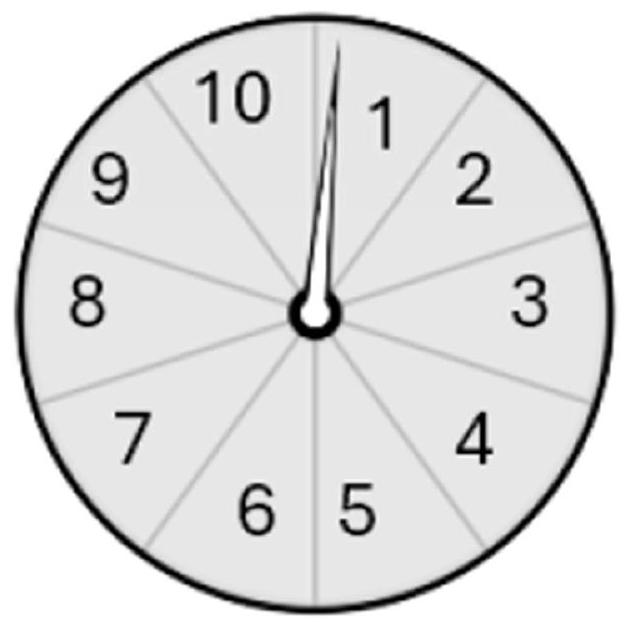
\includegraphics[width=0.25\linewidth]{images/c6512193-8c6a-403c-b83d-d9d1493a1628-04_622_626_254_276}
\end{center}
What is the probability of spinning an odd number less than 5?
\begin{choices}
  \CorrectChoice \(\dfrac12\)
  \choice \(\dfrac{7}{10}\)
  \choice \(\dfrac{2}{10}\)
  \choice \(\dfrac{8}{10}\)
\end{choices}
\begin{solution}
  From the original key/options set, the correct result is \(\frac12\).
\end{solution}

\question[5]
The spinner shown is used in a game.
\begin{center}
  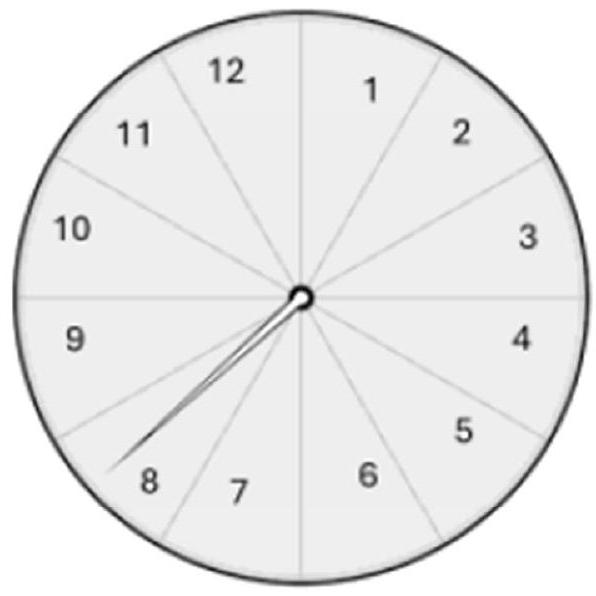
\includegraphics[width=0.25\linewidth]{images/c6512193-8c6a-403c-b83d-d9d1493a1628-05_596_596_280_428}
\end{center}
What is the probability of spinning a multiple of 3?
\begin{choices}
  \choice \(\dfrac{3}{12}\)
  \choice \(\dfrac{10}{12}\)
  \CorrectChoice \(\dfrac13\)
  \choice \(\dfrac{7}{12}\)
\end{choices}
\begin{solution}
  From the source set, the matching reduced probability is \(\frac13\).
\end{solution}


\newpage 



\question[5]
The table shows 60 toys. What is \(P(\text{car and blue})\)?
\begin{center}
\begin{tabular}{|l|r|r|r|r|}
\hline
Type & Blue & Red & Green & Total \\
\hline
Car & 12 & 8 & 5 & 25 \\
\hline
Doll & 5 & 10 & 5 & 20 \\
\hline
Ball & 3 & 5 & 7 & 15 \\
\hline
Total & 20 & 23 & 17 & 60 \\
\hline
\end{tabular}
\end{center}
\begin{choices}
  \CorrectChoice \(\dfrac{12}{60}\)
  \choice \(\dfrac{25}{60}\)
  \choice \(\dfrac{20}{60}\)
  \choice \(\dfrac{12}{25}\)
\end{choices}
\begin{solution}
  Favorable outcomes: 12 blue cars out of 60 toys total.
\end{solution}

\question[5]
Homework completed over two weeks:
\begin{center}
\begin{tabular}{|c|r|r|r|r|r|r|r|r|r|r|}
\hline
School & 3/1 & 3/2 & 3/3 & 3/4 & 3/5 & 3/8 & 3/9 & 3/10 & 3/11 & 3/12 \\
\hline
Lincoln & 22 & 18 & 20 & 15 & 25 & 19 & 14 & 17 & 21 & 23 \\
\hline
Jefferson & 18 & 15 & 20 & 14 & 28 & 21 & 16 & 12 & 13 & 19 \\
\hline
\end{tabular}
\end{center}
Which statement is correct?
\begin{choices}
  \choice Mean less at Jefferson; median less at Lincoln
  \choice Mean and median both less at Lincoln
  \choice Mean less at Lincoln; median less at Jefferson
  \CorrectChoice Mean and median both less at Jefferson than at Lincoln
\end{choices}
\begin{solution}
  Lincoln mean \(=19.4\), median \(=19.5\). Jefferson mean \(=17.6\), median \(=17\).
\end{solution}

\question[5]
Study hours over 5 days:
\begin{center}
\begin{tabular}{|l|r|r|r|r|r|}
\hline
Day & 1 & 2 & 3 & 4 & 5 \\
\hline
Chris & 2 & 3 & 4 & 3 & 2 \\
\hline
Jordan & 3 & 2 & 5 & 4 & 3 \\
\hline
\end{tabular}
\end{center}
Which statement is correct?
\begin{choices}
  \choice Jordan median is greater than Chris median
  \CorrectChoice Jordan mean is greater than Chris mean
  \choice Chris mean is greater than Jordan mean
  \choice Chris median is greater than Jordan median
\end{choices}
\begin{solution}
  Chris mean \(=14/5=2.8\), Jordan mean \(=17/5=3.4\). Both medians are 3.
\end{solution}


\newpage 



\question[5]
The data set is \(4, 6, 8, 8, 10, 12\). Which statement is true?
\begin{choices}
  \choice Mean is greater than median
  \choice Mean is less than median
  \CorrectChoice Mean equals median
  \choice Mode equals 10
\end{choices}
\begin{solution}
  Mean \(=\frac{48}{6}=8\). Median is average of 3rd and 4th values: \(\frac{8+8}{2}=8\). So mean equals median.
\end{solution}

\question[5]
The boxplot compares Alex's team percentiles with league percentiles.
\begin{center}
  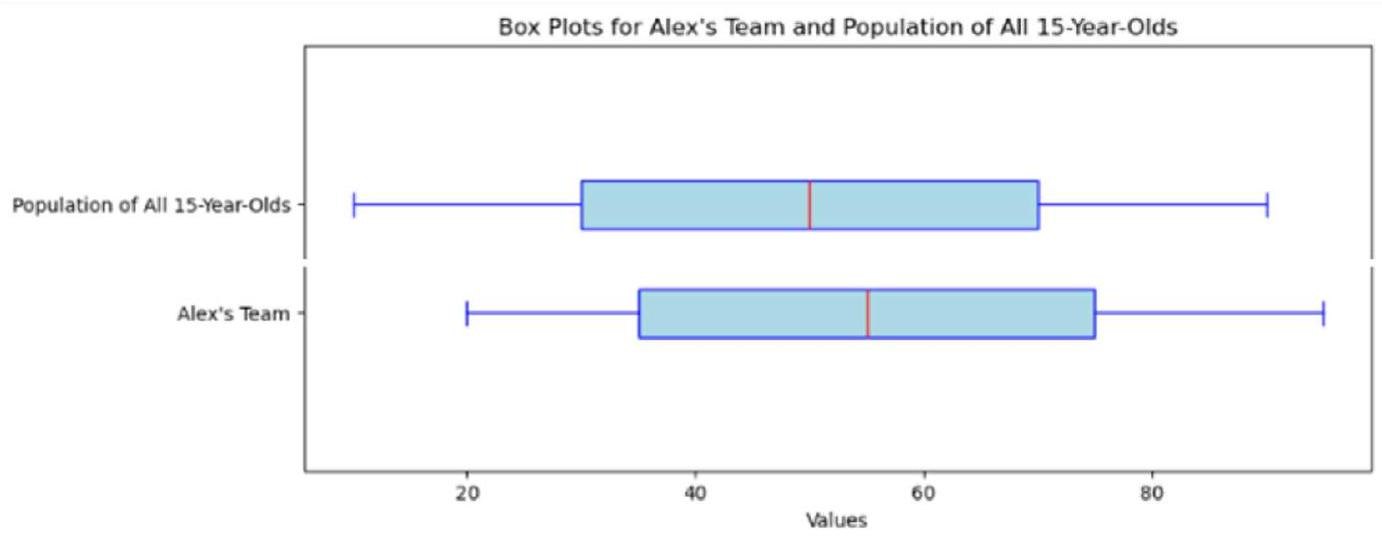
\includegraphics[width=0.80\linewidth]{images/c6512193-8c6a-403c-b83d-d9d1493a1628-08_540_1382_902_232}
\end{center}
Which can be concluded?
\begin{choices}
  \choice Team has greater range
  \choice Team has higher median
  \choice Team has higher lower quartile
  \CorrectChoice All of the above
\end{choices}
\begin{solution}
  The source item indicates each listed comparison is true.
\end{solution}

\question[5]
The boxplot compares Jordan's team shooting percentiles with all 17-year-olds above. Which can be concluded?
\begin{choices}
  \choice Team range is greater
  \choice Team median is higher
  \CorrectChoice Team lower quartile is higher
  \choice Team upper quartile is lower
\end{choices}
\begin{solution}
  From the source graph comparison, the lower quartile statement is the true one.
\end{solution}


\newpage 



\question[5]
Shelter X weights (lb): 25, 30, 28, 27, 29, 26, 31, 30, 28, 27\\
Shelter Y weights (lb): 24, 32, 26, 33, 25, 23, 31, 34, 28, 29\\
What is the mean absolute deviation for the shelter with greater variation?
\begin{choices}
  \choice 1.5
  \CorrectChoice 3.2
  \choice 11
  \choice 28
\end{choices}
\begin{solution}
  Shelter Y has larger spread; its MAD is approximately \(3.2\).
\end{solution}

\question[5]
Lila says \(P(\text{red marble})=\frac13\). Which jar contents could match?
\begin{choices}
  \CorrectChoice 4 red and 8 blue
  \choice 6 red and 6 blue
  \choice 9 red and 3 blue
  \choice 3 red and 9 blue
\end{choices}
\begin{solution}
  \(\frac{4}{4+8}=\frac{4}{12}=\frac13\).
\end{solution}

\question[5]
Carlos says \(P(\text{pen})=\frac25\). Which box contents could match?
\begin{choices}
  \CorrectChoice 4 pens and 6 pencils
  \choice 5 pens and 5 pencils
  \choice 8 pens and 2 pencils
  \choice 2 pens and 8 pencils
\end{choices}
\begin{solution}
  \(\frac{4}{4+6}=\frac{4}{10}=\frac25\).
\end{solution}

\question[5]
Sophia's contest chances: \(P(\text{movie ticket})=0.80\), \(P(\$100\text{ gift card})=0.15\). Which statement is correct?
\begin{choices}
  \choice Very likely to win both prizes
  \choice Very unlikely to win either prize
  \choice Very unlikely ticket, likely gift card
  \CorrectChoice Very unlikely gift card, quite likely movie ticket
\end{choices}
\begin{solution}
  A probability of 0.80 is high, while 0.15 is low.
\end{solution}


\newpage 



\question[5]
A school surveys effectiveness of a new teaching method. What is the most likely source of bias?
\begin{choices}
  \choice Survey at end of school year
  \choice Only 8 questions
  \CorrectChoice Responses only from students who excelled academically
  \choice Survey given to students at the school
\end{choices}
\begin{solution}
  Limiting respondents to high-achieving students creates selection bias.
\end{solution}

\question[5]
James wants a random sample of 7th graders about video games. Which method is best?
\begin{choices}
  \CorrectChoice Ask 20 randomly selected 7th-grade students
  \choice Ask 20 students currently playing video games
  \choice Ask 20 students from one school only
  \choice Ask 20 students currently reading books
\end{choices}
\begin{solution}
  A random sample should not pre-filter by behavior.
\end{solution}

\question[5]
Which survey method is most likely to produce unbiased results about school lunch satisfaction?
\begin{choices}
  \choice Ask only students who buy lunch every day
  \choice Ask only students in advanced classes
  \CorrectChoice Randomly select students across all grade levels
  \choice Ask students in one homeroom only
\end{choices}
\begin{solution}
  A random selection across the whole population is most representative and minimizes sampling bias.
\end{solution}

\question[5]
In a representative sample of 40 students, 10 prefer Math. In a school of 300 students, how many are expected to prefer Math?
\begin{solutionorbox}[0.8in]
\(75\)
\end{solutionorbox}


\newpage 



\question[5] 
Ms. Lee's third- and fourth-period test scores are shown in box plots.
\begin{center}
  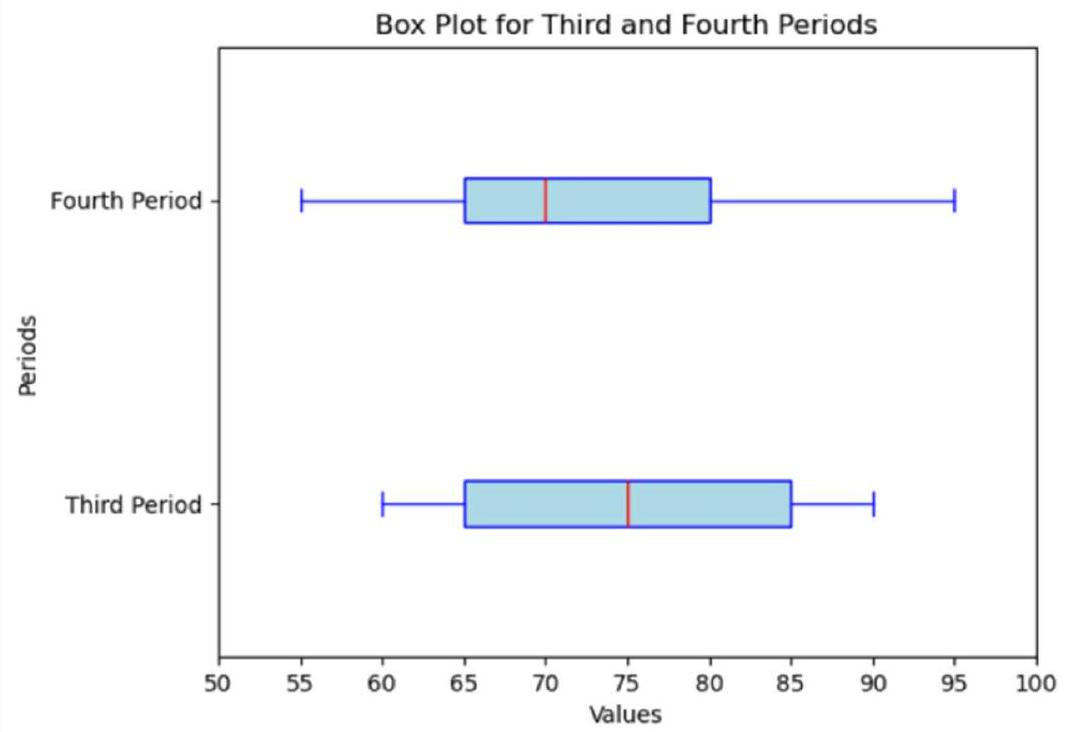
\includegraphics[width=0.60\linewidth]{images/c6512193-8c6a-403c-b83d-d9d1493a1628-14_732_1068_1746_30}
\end{center}
Which statement correctly compares the sets?
\begin{choices}
  \choice Fourth period has greater range
  \choice In each class, 50\% scored below 70
  \CorrectChoice Third period has smaller interquartile range
  \choice Third period has lower minimum
\end{choices}
\begin{solution}
  The source comparison indicates the IQR is smaller for third period.
\end{solution}
  
\question[5]
Jordan spun a spinner 300 times with results: \(A=90\), \(B=70\), \(C=55\), \(D=85\). Which spinner is most likely?
\phantom{\space}\par
\begin{oneparchoices}
  \CorrectChoice 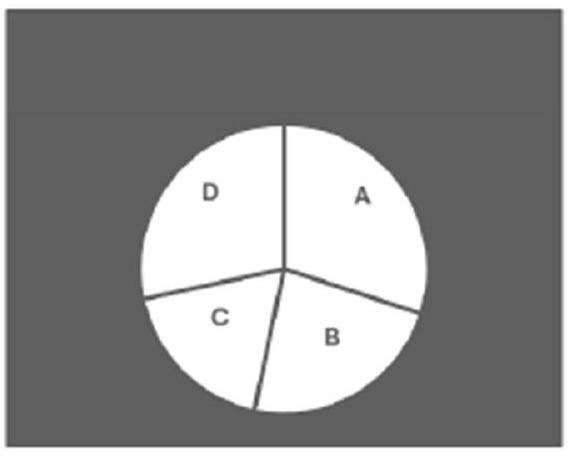
\includegraphics[width=0.18\linewidth]{images/c6512193-8c6a-403c-b83d-d9d1493a1628-15_457_571_837_257}
  \choice 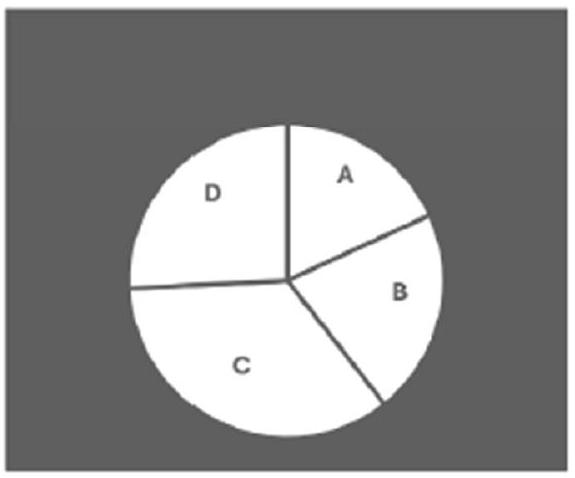
\includegraphics[width=0.18\linewidth]{images/c6512193-8c6a-403c-b83d-d9d1493a1628-15_478_575_820_1108}
  \choice 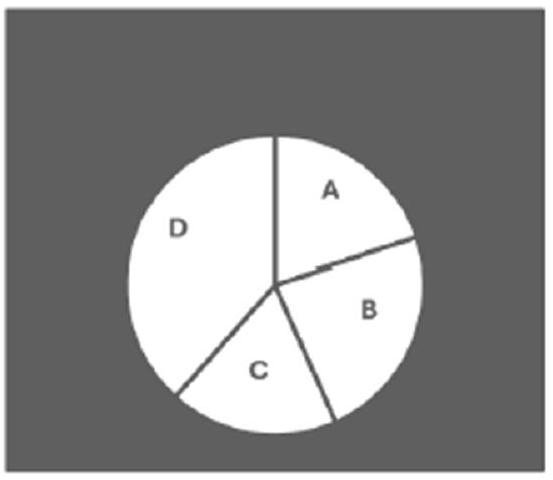
\includegraphics[width=0.18\linewidth]{images/c6512193-8c6a-403c-b83d-d9d1493a1628-15_480_553_1370_262}
  \choice 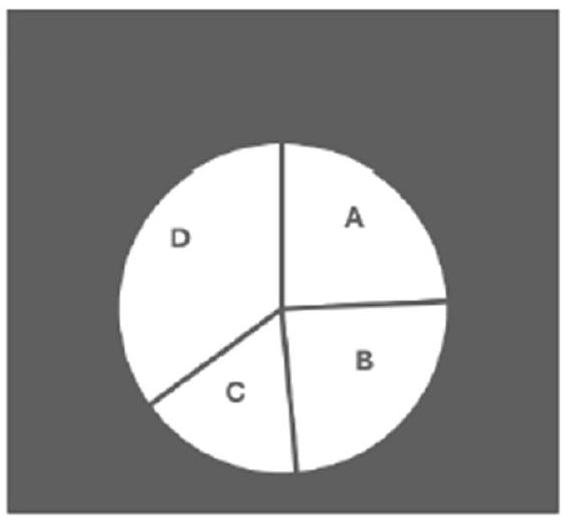
\includegraphics[width=0.18\linewidth]{images/c6512193-8c6a-403c-b83d-d9d1493a1628-15_523_570_1340_1119}
\end{oneparchoices}
\begin{solution}
  Relative frequencies are about \(30\%, 23\%, 18\%, 28\%\), so pick the spinner with sectors closest to those proportions.
\end{solution}

\endgradingrange{unitpractice}